\section{Análisis de la obra pictórica: Cristo de San Juan de la Cruz de Dalí}

\begin{figure}[ht!]
    \centering
    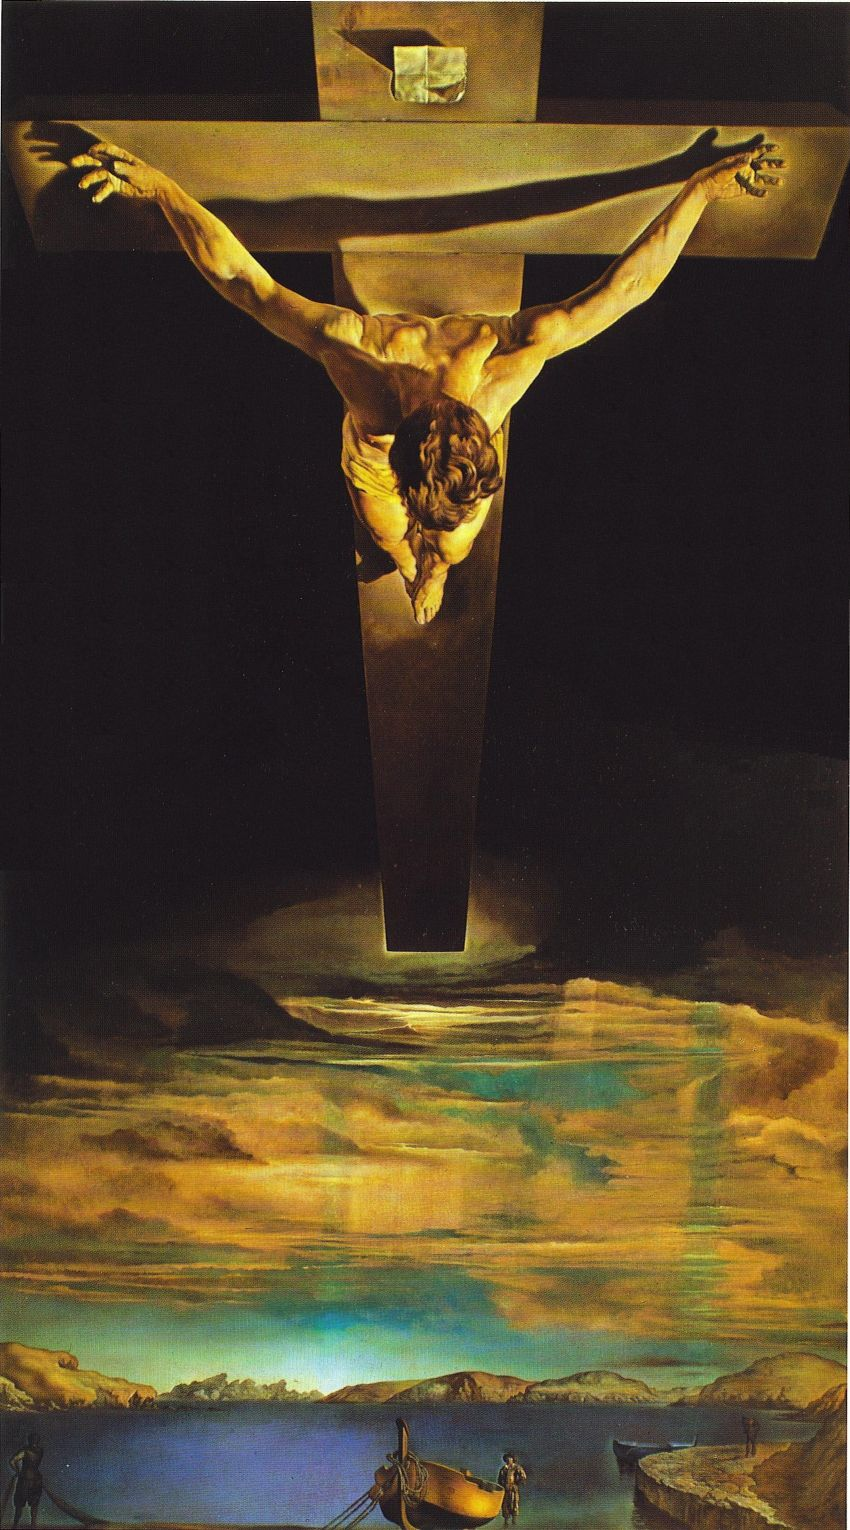
\includegraphics[width=0.84\textwidth]{dali.jpg}
   .\caption{Cristo de San Juan de la Cruz de Salvador Dalí. Museo Kelvingrove.} % URL: blogsantiagosoul.wordpress.com/tag/viva-la-vida}
\end{figure}

\newpage

%Arte, estilo: Surrealismo
%Cronología: 1951
%Lugar: Museo Kelvingrove, Glasgow, Reino Unido
%Autor: Salvador Dalí
%Título: Cristo de San Juan de la Cruz

%Función: Se expuso por primera vez en la galería Lefevre de Londres. %http://www.xn--esarteespaol-jhb.es/contenido.php?recordID=11

\begin{description}
\item[Estilo] Surrealismo
\item[Cronología] 1951
\item[Lugar] Museo Kelvingrove, Glasgow
\item[Autor] Salvador Dalí
\item[Título] Cristo de San Juan de la Cruz
\end{description}

\textbf{Contexto histórico:}

Esta obra se realizó en plena dictadura franquista, en la que numerosos artistas fueron desterrados por no compartir las ideas de la dictadura. No siendo así para Dalí que no sólo aceptó la dictadura franquista, sino que incluso elaboró un retrato de la nieta del propio Franco.

Gran pintor de estilo surrealista, Dalí siguió un estilo propio y más extravagante que el del resto de sus compañeros. El surrealismo nació en 1924, en París a manos de André Breton que publicó el \textit{Primer Manifiesto Surrealista}. Los pintores de esta corriente, influidos enormemente por las teorías de Freud, intentaron expresar en sus obras el mundo del subconsciente.

Dalí enseguida sobresalió en este estilo con una primera etapa más agresiva. Sin embargo, a partir del 1948, cuando regresó a Europa de América, inició una etapa en la que vuelve al clasicismo, reproduciendo sus primeros temas religiosos. Una de estas obras religiosas es la del Cristo de San Juan de la Cruz. Este Cristo está basado, como su nombre indica, en el Cristo dibujado por San Juan de la Cruz tras una revelación(ver anexo \autoref{app:sanjuan}).

Dalí decidió representar \textit{un Cristo bello como el mismo Dios que él encarna} y no centrase en la fealdad para provocar la emoción en el espectador. Lo hizo adoptando una perspectiva totalmente nueva de la crucifixión. Con este nuevo enfoque situó a Cristo en la Cruz en una posición vertical y casi perpendicular al espectador de la obra.

Además decidió retirar todos aquellos elementos que intervinieron en la crucifixión de Cristo, nótese que éste no conserva la corona de espinas ni ninguna herida, tampoco están dibujados los clavos que lo deberían sostener en la cruz, en la que parece que está suspendido por arte de magia.

Debajo de la imagen principal del cuadro se puede apreciar un paisaje, supuestamente representado a partir de la bahía de Port Lligat. En ella se ven dos pescadores que, sin embargo, están inspirados en los pintores Le Nain y Velazquez.

El Cristo se sitúa en un fondo oscuro que le da una imagen dramática a la obra junto al contraste con la iluminación que se proyecta en forma de rayo de luz sobre la figura. Entre la imagen del crucificado y la de los pescadores se interpone un cielo nuboso, que aporta a la obra aún mayor dramatismo al separar la crucifixión y la imagen de la tranquila bahía de pescadores, dando a entender la indiferencia de éstos ante el suceso que se está produciendo.

% http://www.artehistoria.jcyl.es/v2/obras/9639.htm
% http://unapizcadecmha.blogspot.com.es/2013/11/el-cristo-de-san-juan-de-la-cruz-1951.html
% http://www.arteespana.com/salvadordali.htm
% Artículo de San Juan de la Cruz
% libro de aita

\vspace{12pt}
\textbf{Anatomía de superficie:}

En esta obra en la que Dalí refleja una nueva perspectiva de la crucifixión de Cristo, siendo la cabeza de éste el centro de la obra, podemos observar un Cristo de con características totalmente diferentes a las apreciadas en la mayoría de obras acerca de la crucifixión. Aparte de tener el pelo corto, al contrario que en las numerosas obras en las que se representa a Cristo, no posee signos de sufrimiento, ni clavos que le sujeten a la cruz, ni corona de espinas, ni tampoco sangre puesto que no hay heridas de las que pueda brotar.

Aún sin elementos de crucifixión la figura mantiene una posición en la que se sugiere que ambos pies estarían unidos a la cruz mediante el mismo clavo, mientras que los clavos de las extremidades superiores se encontrarían en las palmas de las manos. Esto último se puede percibir en la caída del cuerpo hacia delante que ocurre desde más arriba de las muñecas, según la sombra que se proyecta detrás.

Al estar la cabeza inclinada hacia delante, no es posible ver el resto del cuerpo de la figura, sin embargo si ofrece una visión espectacular de la espalda y de sus músculos. Los brazos caen extendidos, formando un triángulo con la cruz que mantiene suspendido a Crsito y dando una sensación de que éste se encuentra colgado boca abajo por el espacio que hay entre su cuerpo y la cruz.

El autor en esta obra de arte no se centra en el sufrimiento y la muerte de Cristo, sino que intenta evocar la belleza de Cristo Dios. Por ello se puede considerar admirable la simetría del cuerpo y la anatomía que se vislumbra. La actitud de la figura es relajada, pudiéndose observar este hecho en la posición de sus brazos y de los músculos de la espalda.

No es posible saber si el Cristo se encuentra fellecido o al borde de serlo en la obra, puesto que el autor ilumina la figura con una luz amarillenta que crea un gran contraste entre las zonas iluminadas y las zonas en sombra y no deja observar el verdadero color del cuerpo de la figura.

Diferentes estructuras anatómicas se pueden observar en esta obra de acuerdo a la perspectiva y posición de la figura, que no coinciden con las descritas en figuras anteriores.

Los músculos de la espalda y los de la parte posterior del cuello, aunque totalmente relajados, son claramente visibles. Sin embargo el claroscuro utilizado por el autor dificulta la identificación de estos.

La línea del ligamento nucal que recorre las vertebras cervicales si se observa, no identificando de manera correcta las apófisis espinosas de las vertebras cervicales inferiores, especialmente la de la C7, que por la postura tendrían que ser fácilmente visibles. 

La masa muscular del cuello la componen el músculo esplenio, el músculo esternocleidomastoideo y el trapecio, que se inserta superiormente en la línea nucal superior y también ocupa gran espacio de la espalda.

En la espalda, cubiertas por el músculo trapecio, se perciben las siluetas de las escápulas. Éste músculo junto con  el serrato anterior, que no es visible en la figura, realiza la rotación externa de las escápulas, necesaria en la posición adoptada por la figura de la obra.

En la masa muscular de los brazos se aprecian los deltoides que son los principales músculos abductores del brazo, recubriendo el hombro. Además de extendido el brazo está en posición de supinación. De la extensión se encarga el tríceps braquial, mientras que la supinación requiere de la acción del músculo braquiorradial, que se encuentra en el antebrazo. Las manos se encuentran en posición de descanso, apreciando cierta flexión de las articulaciones interfalángicas y metacarpofalángicas provocada por los músculos flexor carpi radialis, palmar mayor, flexor superficial de los dedos y flexor carpi ulnaris que pasan del antebrazo a la mano.

Anteriormente se aprecia el músculo pectoral mayor que forma el pliegue anterior de la axila. Sin embargo ésta no se ve, puesto que queda tapada por el hombro y su propio pliegue anterior.

El tórax, abdomen, pelvis y parte de la extremidades inferiores están ocultas por la cabeza, que cae hacia delante. únicamente podemos apreciar parte del muslo, las articulaciones de las rodillas y los pies, diminutos debidos a la perspectiva. La principal masa muscular del muslo es el cuadriceps, cuya función es la extensión de la rodilla, el borde lateral del muslo lo forma el músculo sartorio, el cual nos permite cruzar las piernas. Ambos movimientos imprecindibles para la postura de Cristo con ambas piernas extendidas y crucificado con un pie encima del otro.

Sin embargo, la articulación de la rodilla de la pierna izquierda, está ligeramente flexionada para permitir que el pie de esta extremidad pueda situarse encima del pie de la extremidad derecha. La flexión de la rodilla está realizada por varios músculos: los isquiotibiales, el sartorio, el poplíteo y los gemelos.
